\documentclass[journal]{vgtc}                % final (journal style)
%\documentclass[review,journal]{vgtc}         % review (journal style)
%\documentclass[widereview]{vgtc}             % wide-spaced review
%\documentclass[preprint,journal]{vgtc}       % preprint (journal style)

%% Uncomment one of the lines above depending on where your paper is
%% in the conference process. ``review'' and ``widereview'' are for review
%% submission, ``preprint'' is for pre-publication, and the final version
%% doesn't use a specific qualifier.

%% Please use one of the ``review'' options in combination with the
%% assigned online id (see below) ONLY if your paper uses a double blind
%% review process. Some conferences, like IEEE Vis and InfoVis, have NOT
%% in the past.

%% Please note that the use of figures other than the optional teaser is not permitted on the first page
%% of the journal version.  Figures should begin on the second page and be
%% in CMYK or Grey scale format, otherwise, colour shifting may occur
%% during the printing process.  Papers submitted with figures other than the optional teaser on the
%% first page will be refused. Also, the teaser figure should only have the
%% width of the abstract as the template enforces it.

%% These few lines make a distinction between latex and pdflatex calls and they
%% bring in essential packages for graphics and font handling.
%% Note that due to the \DeclareGraphicsExtensions{} call it is no longer necessary
%% to provide the the path and extension of a graphics file:
%% 
\includegraphics{diamondrule} is completely sufficient.
%%
\ifpdf%                                % if we use pdflatex
  \pdfoutput=1\relax                   % create PDFs from pdfLaTeX
  \pdfcompresslevel=9                  % PDF Compression
  \pdfoptionpdfminorversion=7          % create PDF 1.7
  \ExecuteOptions{pdftex}
  \usepackage{graphicx}                % allow us to embed graphics files
  \DeclareGraphicsExtensions{.pdf,.png,.jpg,.jpeg} % for pdflatex we expect .pdf, .png, or .jpg files
\else%                                 % else we use pure latex
  \ExecuteOptions{dvips}
  \usepackage{graphicx}                % allow us to embed graphics files
  \DeclareGraphicsExtensions{.eps}     % for pure latex we expect eps files
\fi%

%% it is recomended to use ``\autoref{sec:bla}'' instead of ``Fig.~\ref{sec:bla}''
\graphicspath{{figures/}{pictures/}{images/}{./}} % where to search for the images

\usepackage[utf8]{inputenc}
\usepackage{microtype}                 % use micro-typography (slightly more compact, better to read)
\PassOptionsToPackage{warn}{textcomp}  % to address font issues with \textrightarrow
\usepackage{textcomp}                  % use better special symbols
\usepackage{mathptmx}                  % use matching math font
\usepackage{times}                     % we use Times as the main font
\renewcommand*\ttdefault{txtt}         % a nicer typewriter font
\usepackage{cite}                      % needed to automatically sort the references
%\usepackage{color}
\usepackage{xcolor} % Some more colors not defined in "color" package
% \usepackage{tabu}                      % only used for the table example
% \usepackage{booktabs}                  % only used for the table example
\usepackage{todonotes}
\usepackage[draft]{hyperref} % Weeeeird error occurs without this.


\newcommand{\kallecomment}[1]{\textbf{[-Kalle-~}
    \textcolor{orange}{#1}
    \textbf{~]}}

\newcommand{\emilcomment}[1]{\textbf{[-Emil-~}
    \textcolor{red}{#1}
    \textbf{~]}}

\newcommand{\alexcomment}[1]{\textbf{[-Alex-~}
    \textcolor{magenta}{#1}
    \textbf{~]}}

\newcommand{\anderscomment}[1]{\textbf{[-Anders-~}
    \textcolor{cyan}{#1}
    \textbf{~]}}

\newcommand{\etal}{\emph{et~al.}}


%% We encourage the use of mathptmx for consistent usage of times font
%% throughout the proceedings. However, if you encounter conflicts
%% with other math-related packages, you may want to disable it.

%% In preprint mode you may define your own headline.
%\preprinttext{To appear in IEEE Transactions on Visualization and Computer Graphics.}

%% If you are submitting a paper to a conference for review with a double
%% blind reviewing process, please replace the value ``0'' below with your
%% OnlineID. Otherwise, you may safely leave it at ``0''.
\onlineid{0}

%% declare the category of your paper, only shown in review mode
\vgtccategory{Research}
%% please declare the paper type of your paper to help reviewers, only shown in review mode
%% choices:
%% * algorithm/technique
%% * application/design study
%% * evaluation
%% * system
%% * theory/model
\vgtcpapertype{System}

%% Paper title.

\title{Globe Browsing: Contextualized Spatio-Temporal Planetary Surface Visualization}

%% This is how authors are specified in the journal style

%% indicate IEEE Member or Student Member in form indicated below
\author{Karl Bladin, Emil Axelsson, Erik Broberg, Carter Emmart, Patric Ljung, \\ Alexander Bock and Anders Ynnerman, \textit{Associate Member, IEEE}}
\authorfooter{
%% insert punctuation at end of each item
\item
 Karl Bladin, Emil Axelsson, Patric Ljung, Anders Ynnerman and Erik Broberg are with Linköping University.
 E-mail: \{ karl.bladin, emil.axelsson, patric.ljung, anders.ynnerman \} @liu.se, erikbr049@student.liu.se
 \item
 Carter Emmart is with American Museum of Natural History. E-mail: carter@amnh.org.
 \item
 Alexander Bock is with New York University. E-mail alexander.bock@nyu.edu
}

%other entries to be set up for journal
\shortauthortitle{Bladin \MakeLowercase{\textit{et al.}}: Globe Browsing}

%% Abstract section.
\abstract{%
We present work on tailoring and integration of multiple data processing and visualization methods to interactively contextualize geospatial data of celestial bodies for use in public science dissemination and communication between domain scientists.
Results of planetary mapping is often shared openly for use in scientific research and mission planning.
However, this data is, in its raw format, not accessible to non-experts, as it is difficult to grasp the context of the data and the intricate acquisition process.
As our approach is full interactive and handles dynamic data sources, we are significantly shortening the time between discovery and dissemination of data and results.
We describe the image acquisition, required pre-processing steps to derive a 2.5D terrain, and a chunked level-of-detail, out-of-core rendering approach to enable interactive exploration of global maps as well as high-resolution digital terrain models.
One interesting case is Mars as extensive amount of map data is available from various missions.
A second case is dynamical processes, such as weather conditions on Earth that require spatio-temporal datasets.
In addition to visualizing the scientific results, we also present ongoing data acquisition, exemplified in the Pluto flyby of the New Horizons spacecraft.
Our work has been implemented in the OpenSpace software, which enables interactive presentations in a range of environments such as immersive dome theaters and virtual reality headsets.

%
% In addition, the application supports temporal datasets, where available, in order to visualize a celestial body's dynamic processes, such as weather conditions on Earth.
% Furthermore, we interactively play back in-situ visualizations of the process for data acquisition.
%
%
%We present an application where scientific mapping data of celestial bodies is contextualized in space and time to enrich the experience in public dissemination as well as to support communication between scientists.
%In our system various types of datasets and visualization techniques are combined.
%A chunked level-of-detail approach is used to enable interactive exploration of global maps as well as local high-resolution digital terrain models with textures and height information.
%This is particularly interesting for Mars thanks to the extensive amount of map data gathered by the various missions to this planet.
%Using time varying data sets, we visualize the dynamics of a celestial body, such as weather conditions on Earth.
%Furthermore, we interactively play back in-situ visualizations of the process for data acquisition.
%
%Our work has been implemented in the open source software OpenSpace, which enables interactive presentations in immersive environments like dome theaters and virtual reality headsets.
%
%
%
%
%
%The mapping of the planets and moons within our solar system is carried out by space organizations such as NASA and ESA.
%Image data are collected by cameras on satellites and spacecrafts, and used in scientific research and in planning of future space missions.
%Despite the fact that NASA shares a lot of its image data openly, it seldom reaches the general public.
%
%A lot of research has been done in terms of visualizing planetary data using terrain rendering. Current technology relies on techniques such as out-of-core, and dynamic level of detail rendering, multi threaded data acquisition and consideration of precision limitations.
%
%These systems are often either specialized for researchers where accuracy is the main concern, or for games, where the user experience plays a major role.
%
%We present an application for visualizing the same data that space scientists analyze in the context of a virtual environment representing the space that we are exploring.
%Given the contextualization that the real space provides, we can model the solar system using positional data for modelling the planets' orbits together with the space probes that explores them.
%In a time varying visualizations we can show the dynamics of a planetary surface as well as the data collection process itself.
%
%The main focus of this paper is to describe the combination of different datasets gathered for mapping out planets' surface features. 
% particularly Mars due to the extensive amount of map data gathered by the various missions on this planet.
%
%Our rendering system combines various resolutions of local and global map datasets and presents them together in their real context.
%Using the Geospatial Data Abstraction Library (GDAL), we can preprocess images to match the most common cylindrical projection format used for globe rendering.
%A chunked level of detail approach is used for rendering tiles which are height mapped on the fly.
%This allows for a versatile globe renderer which can easily load new datasets without requiring preprocessing by the rendering software.
%
%We can use the same data that scientists use in their research for public dissemination and present it, bundled and contextualized, using immersive rendering systems.
%Our software, OpenSpace, is an open source project with the goal of bringing space science to the general public.
%
%
% The mapping of the planets and moons within our solar system is carried out by space organizations such as NASA and
% ESA. Image data are collected by instruments on satellites and spacecrafts, and subsequently used in scientific research and mission
% planning. While map data from space missions are often shared openly, it can be difficult for non-experts to comprehend the context of
% the data and understand the acquisition process.
% We present an application where scientific mapping data of celestial bodies is contextualized in space and time to enrich the experience
% in public dissemination as well as to support communication between scientists. In our system various types of datasets and
% visualization techniques are combined; A chunked level-of-detail approach is used to enable interactive exploration of global maps as
% well as local high-resolution digital terrain models with textures and height information. This is particularly interesting for Mars thanks
% to the extensive amount of map data gathered by the various missions to this planet. Using time varying data sets, we visualize the
% dynamics of a celestial body, such as weather conditions on Earth. Furthermore, we interactively play back in-situ visualizations of the
% process for data acquisition.
% Our work has been implemented in the open source software OpenSpace that enables interactive presentations in immersive
% environments like dome theaters and virtual reality headsets.
%
%
} % end of abstract

%% Keywords that describe your work. Will show as 'Index Terms' in journal
%% please capitalize first letter and insert punctuation after last keyword
\keywords{Astronomical visualization, globe rendering, public dissemination, science communication, space mission visualization }

%% ACM Computing Classification System (CCS). 
%% See <http://www.acm.org/class/1998/> for details.
%% The ``\CCScat'' command takes four arguments.

\CCScatlist{ % not used in journal version
 \CCScat{K.6.1}{Management of Computing and Information Systems}%
{Project and People Management}{Life Cycle};
 \CCScat{K.7.m}{The Computing Profession}{Miscellaneous}{Ethics}
}

%% Uncomment below to include a teaser figure.
\teaser{
  \centering
  %\includegraphics[width=\linewidth]{CypressView}
  %\caption{In the Clouds: Vancouver from Cypress Mountain. Note that the teaser may not be wider than the abstract block.}
%	\label{fig:teaser}
}

%% Uncomment below to disable the manuscript note
%\renewcommand{\manuscriptnotetxt}{}

%% Copyright space is enabled by default as required by guidelines.
%% It is disabled by the 'review' option or via the following command:
% \nocopyrightspace

\vgtcinsertpkg

%%%%%%%%%%%%%%%%%%%%%%%%%%%%%%%%%%%%%%%%%%%%%%%%%%%%%%%%%%%%%%%%
%%%%%%%%%%%%%%%%%%%%%% START OF THE PAPER %%%%%%%%%%%%%%%%%%%%%%
%%%%%%%%%%%%%%%%%%%%%%%%%%%%%%%%%%%%%%%%%%%%%%%%%%%%%%%%%%%%%%%%%

\begin{document}

%% The ``\maketitle'' command must be the first command after the
%% ``\begin{document}'' command. It prepares and prints the title block.

%% the only exception to this rule is the \firstsection command
\firstsection{Introduction} \label{sec:introduction}
\maketitle
\kallecomment{Maybe some more catchy name of the article? "Browsing the Red Planet", "Browsing Mars", "Unveiling Mars"? :P}
\emilcomment{Public dissemination of celestial bodies using spatial-temporal mapping-data ?}
\anderscomment{Spatio-temporal planetary surface data capture, mapping and visualization, 
Immersive visualisation of spatio-temporal planetary surface data capture and mapping ?}


\begin{enumerate}
\item Visualizing space data is important because its expensive

\kallecomment{What is expensive?}

\item There exists a vast amount of data from Mars orbiters

The amount of open data currently available from space missions is extensive.
... \kallecomment{Information on the amount of open data from for example NASA.}

NASA's Viking program, launched in the year 1975, gathered important information about Mars and its surface features from the two orbiting satellites and the landers put on the surface of the planet.
Today, the most important large scale imaging campaign on the planet is carried out by the Mars Reconnaissance Orbiter (MRO).
This satellite carries the MARCI (Mars Color Imager), CTX (Context Camera) and HiRISE (High Resolution Imaging Science Experiment) cameras which are used to image the surface at different resolutions \cite{mromission}.

Our goal is to bring space science to the public as well as to provide tools for scientists to talk about space research.
Part of this relies on the ability to visualize planetary science by providing an accurate representation of the globes in our solar system as well as the ability to go there virtually, using the open data available from various space missions.

Raw image data, gathered from space missions, are easily rendered flat on screen. Depending on usage, the images are defined in different projections.
The ground truth is to render images in situ, to recreate the landscapes and build a virtual representation of the actual globes.
It also gives intuitive understanding of how the data is collected by satellites such as the MRO if the images can be rendered in the right context.

Using the tools that scientific data visualization allows, it is possible to get a better understanding of the space missions.
By allowing contol of time flow, showing satellites and space probes in the same context as the planets, and doing this using immersive display systems gives intuitive understanding of the space around us and how scientists gather knowledge about it.

Typical examples of use cases for interactive visualization are large scale dome presentations of real time presentations, virtual reality headsets, and touch tables; where the audience can experience flight through space and time, experiencing our current mapping of the cosmos.

\item Stereoscopic reconstruction from multiple image passes

\kallecomment{Maybe not suitable to put here already?}

\item What datasets are available (Viking, MOLA, CTX, HiRISE) and whats their resolutions

The Mars Global Digital Image Mosaic (MDIM) is a global image dataset with a resolution of 256 pixels/degree \cite{MDIM2.1_web}.
The latest version of this image mosaic, MDIM 2.1 is compiled using a network of images from the Mariner 9 and Viking Orbiters with improved accuracy as a result of constraining control points from the Mars Orbiter Laser Altimeter (MOLA) data \cite{MDIM2.1}.
The dataset is tied to the IAU/IAG 2000 coordinate system which has been adopted by the majority of Mars missions and instrument teams \cite{MDIM2.1}.

The Mars Orbiter Laser Altimeter (MOLA) is an instrument on the Mars Global Surveyor (MGS) spacecraft.
The digital elevation model (DEM), assembled from MOLA data, maps each position on the globe with an offset from the Areoid, Mars' reference ellipsoid, to an average horizontal accuracy of ~100 meters \cite{MOLA}. The dataset has a resolution of 463.0836 meters/pixel \cite{MOLA}.

The HiRISE Operations Center provides images from the HiRISE mission. These are grayscale images, infrared, green and blue images mapped to the red green and blue channels, stereo pairs and digital terrain models generated from stereo pairs.

\kallecomment{Other datasets? Does ESA have Mars missions of interest?}

\kallecomment{GIBS temporal datasets}

\item How can this be applied to other planets, A system for enabling future research thati s correctly contextualized. What is the science question // What is the point of this

By enabling the ability to read many types of image datasets, with global or local coverage, temporal or static, and doing so dynamically, we can generalize the technique to different globes without having a specific focus group.
We hope that our tools can be useful both for scientists who want to present their work in a contextualized manner and for people who find interest in the subjects we discuss or want to experience the most accurate representation of standing on the surface of Mars using only real data.

\end{enumerate}
Length: About 1 page

\section{Related Work} \label{sec:relatedwork}
Our application builds on previous work in the fields of geographical information systems (GIS), level-of-detail (LOD) rendering, large-scale astronomical visualization, as well as visual learning and communication.

\kallecomment{Not sure how much (if anything) we should talk about GIS. Any ideas?}

\textbf{GIS - }Geographical Information Systems relies heavily on the ability to gather, transform, and visualize data with geospatial information.
Maps and DEM's are typical examples of such data and research and development of software solutions to handle different parts of GIS, such as rendering, have lead to different applications in space visualization.

\kallecomment{Can Carter write something here? What other relevant softwares, like Google Mars, are in use?}

\textbf{LOD rendering - } 

Cozzi and Ring (ref) gives a thorough description of the most common methods used for globe rendering today.
Older level of detail techniques such as Real Time Optimally Adaptive Mesh (ROAM) does not allow full GPU throughput and gives way for techniques such as chunked level of detail and geometry clipmaps.




%\subsection{Rendering}

%A globe rendering system needs to handle out of core rendering and level of detail management to avoid flooding the data caches and rendering times.

%Cozzi and Ring (ref) gives a thorough desciription of the most common methods used for globe rendering today. 

%\subsection{3D Reconstruction From Images}

Adding the third dimension required for terrain rendering is most commonly carried out by rendering DTMs, also known as heigh mapping.
Height map datasets can be generated using measured data from altimeters on the satellites, corrected to match an offset from a reference ellipsoid (ref) in the direction of the geodetic normal for every point on the surface covered by the dataset (ref).
Height maps can also be generated using stereoscopic reconstruction.

\textbf{Large scale differences - } The challenges of interactive navigation and positioning in visualizations of large scale environments have been addressed in previous work such as the ScaleGraph by Klashed et al [ref] and Dynamic Scene Graph proposed by Axelsson et al [ref].

\kallecomment{Someone wants to add text about stereo reconstruction here?}

\subsection{Geospatial Data Abstraction}

Geospatial Data Abstraction Library (GDAL) is an open source software package and C++ library enabling re-projection and warping of map datasets and can act as a layer of abstraction between the rendering software and the many different types of map formats and projections.

\begin{enumerate}
\item the book

\kallecomment{3D Engine Design for Virtual Globes?}

\item terrain renderer
\item 3d reconstruction from images (stereoscopic and structure-from-motion)
\item GDAL
\item ``virtual presence'' systems
\item What else?
\end{enumerate}
Length: About 1 page\\
Note:  The page limit was increased to 9+2 pages this year (= 9 pages of manuscript, 2 pages of references). So we should make use of this and cite the hell out of everything that's related

\section{Overview} \label{sec:overview}

\alexcomment{Length: About 2 pages}

\kallecomment{Describe figure shortly:}

\begin{figure}[h]
  \centering
    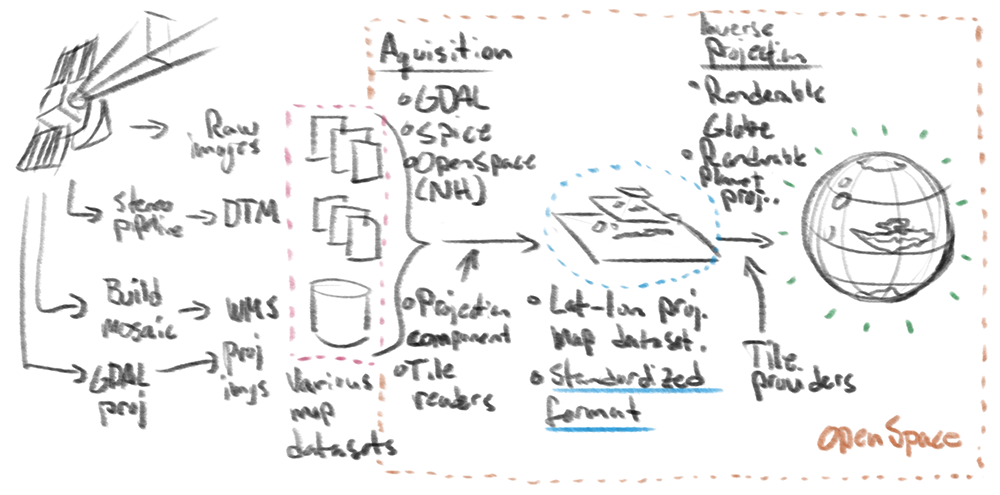
\includegraphics[width=0.5\textwidth]{figures/globe_browsing_data.png}
  \caption{Overview of data flow.}
\end{figure}

\kallecomment{Image (obviously) needs to be updated. Also some rearrangements might be needed. Like better define what part is the actual "acquisition process".}

For versatility we choose to standardize the use of a specific georeferenced map projection format; namely the equirectangular geographic projection, also know as simple cylindrical projection.
This is by far the most commonly supported format used for unprojection of globes.
We want to be able to read as many datasets as possible and avoid heavy preprocessing steps such as reprojection and the need of storing terabytes of reprojected map data.
The geographic projection suffers from a couple of issues near the poles such as oversampling and polar pinching so our globe rendering system works best for regions farther from the poles.

The main task of the acquision process is to gather data and project it to the commonly used geographic format.

Once the image data is in the correct georeferenced coordinate system, the renderer takes care of unprojecting the map to result it the correct mapping of the globe.
This is done using an inverse projection $(x,y,z)^T = P^{-1}(\phi, \theta)$ which maps each geodetic cooridnate defined by a latitude ($\phi$), and a longitude ($\theta$) to a Cartesian coordinate on the surface of the ellipsoid in the model space of the globe (ref either globe book or master thesis).

\kallecomment{MRO -> image datasets}

\kallecomment{image datasets -> DTM (stereo pipeline)}

\kallecomment{reprojection (GDAL)}

\kallecomment{Describe this:}

Image data in some projection format $->$(project)$->$ image data in lonlat projection $->$(render on ellipsoid)$->$ image data ``in-situ'', rendered globe

\section{Image Acquisition and Processing} \label{sec:imageacquisitionprocessing}
\begin{enumerate}
  \item MRO information, different resolution levels
  \item What are the available data products
  \item Ames stereo pipeline
  \item GDAL preprocessing


If the projection format of the images we want to show is not specified, either in a cylindrical projection for the globe in question, or in relation to the space craft that takes the images together with image times, we introduce a preprocessing step to get the right projection format.
In particular, specifying a longitude-latitude projection is necessary to be able to read the map using OpenSpace.
This is easily done by calling the command line application \texttt{gdalwarp}, with the argument \texttt{-t\_srs "+proj=longlat"}.

Sometimes, depending on the dataset we want to render, we want the ability to mask out certain values, transform them, or respecify formats or datatypes.
This can be useful when reading local DTM patches which need to match the underlying height layer.
We use a GDAL feature called virtual datasets which adds an abstraction layer between the actual dataset and the data that comes out when reading using GDAL.

\item WMS

To standardize web requests for map data, the Open GIS Consortium (OGC) specified a web map service interface (ref) and from that, specifications of several other map service interfaces have followed.
The most common standards are Web Map Service (WMS), Tile Map Service (TMS) and Web Map Tile Service (WMTS). Some other, more specific, examples of WMS-like services are WorldWind, VirtualEarth and AGS.

Again using GDAL, we read WMS datasets from remote servers which are specified in the equirectangular geographic projection format.
  
  \item Spice + raw images to lat long \emilcomment{todo.}
\end{enumerate}
Length: About 1-1.5 pages

\section{Rendering System} \label{sec:renderingsystem}

\alexcomment{Length: About 2-2.5 pages (fill as much as the page limit (9+2) allows)}


When the image datasets are in the format required for the renderer, that is defined in a latitude-longitude georeferenced projection, there are several abstraction layers we employ to handle the out of core techniques required for rendering.

\kallecomment{Unsure about the detail level to put on describing things related to the structuring and ownerships of classes etc...}

A renderable globe is an entity in the scene graph structure of OpenSpace.
It consists of a reference ellipsoid definition, a layer manager and a chunked LOD globe.
A layer works much like in image editing softwares and belongs to a specific layer group, these are analogous to blending options.
Examples of layer groups are: height layers, color layers, grayscale layers or grayscale overlays.
The chunked LOD globe takes care of updating the chunk tree and evaluating the levels of its nodes.
It also performs chunk culling as well as rendering of individual chunks.
The chunk renderer has access to a skirted grid (ref) which can be mapped on to a geodetic region and rendered in place using one or several layers for texturing or height mapping.

Other than chunks, a very important concept in the rendering system is the tile.
A tile has a texture representing a geodetic area and is uniquely defined by a layer and a tile index.
A tile index is defined by a level, x, and y coordinates in the chunk tree structure.

\subsection{Reading and Tiling Image Data}

Each layer corresponds to its own ``tile provider''.
A tile provider is able to initiate asynchronous calls to a raw tile data reader which in turn reads the image data from disk or from remote servers.
The raw tile data reader takes as input a tile index and outputs a raw tile that covers the given geographic area with pixels.
Once the image data is ready, a tile can be created on the main thread, uploaded to GPU memory, and pushed in to an in memory LRU cache so that the tile provider can return it upon request.
If the tile is already in the cache, the tile provider simply needs to return it and update the cache upon request.

\begin{figure}[h]
  \centering
    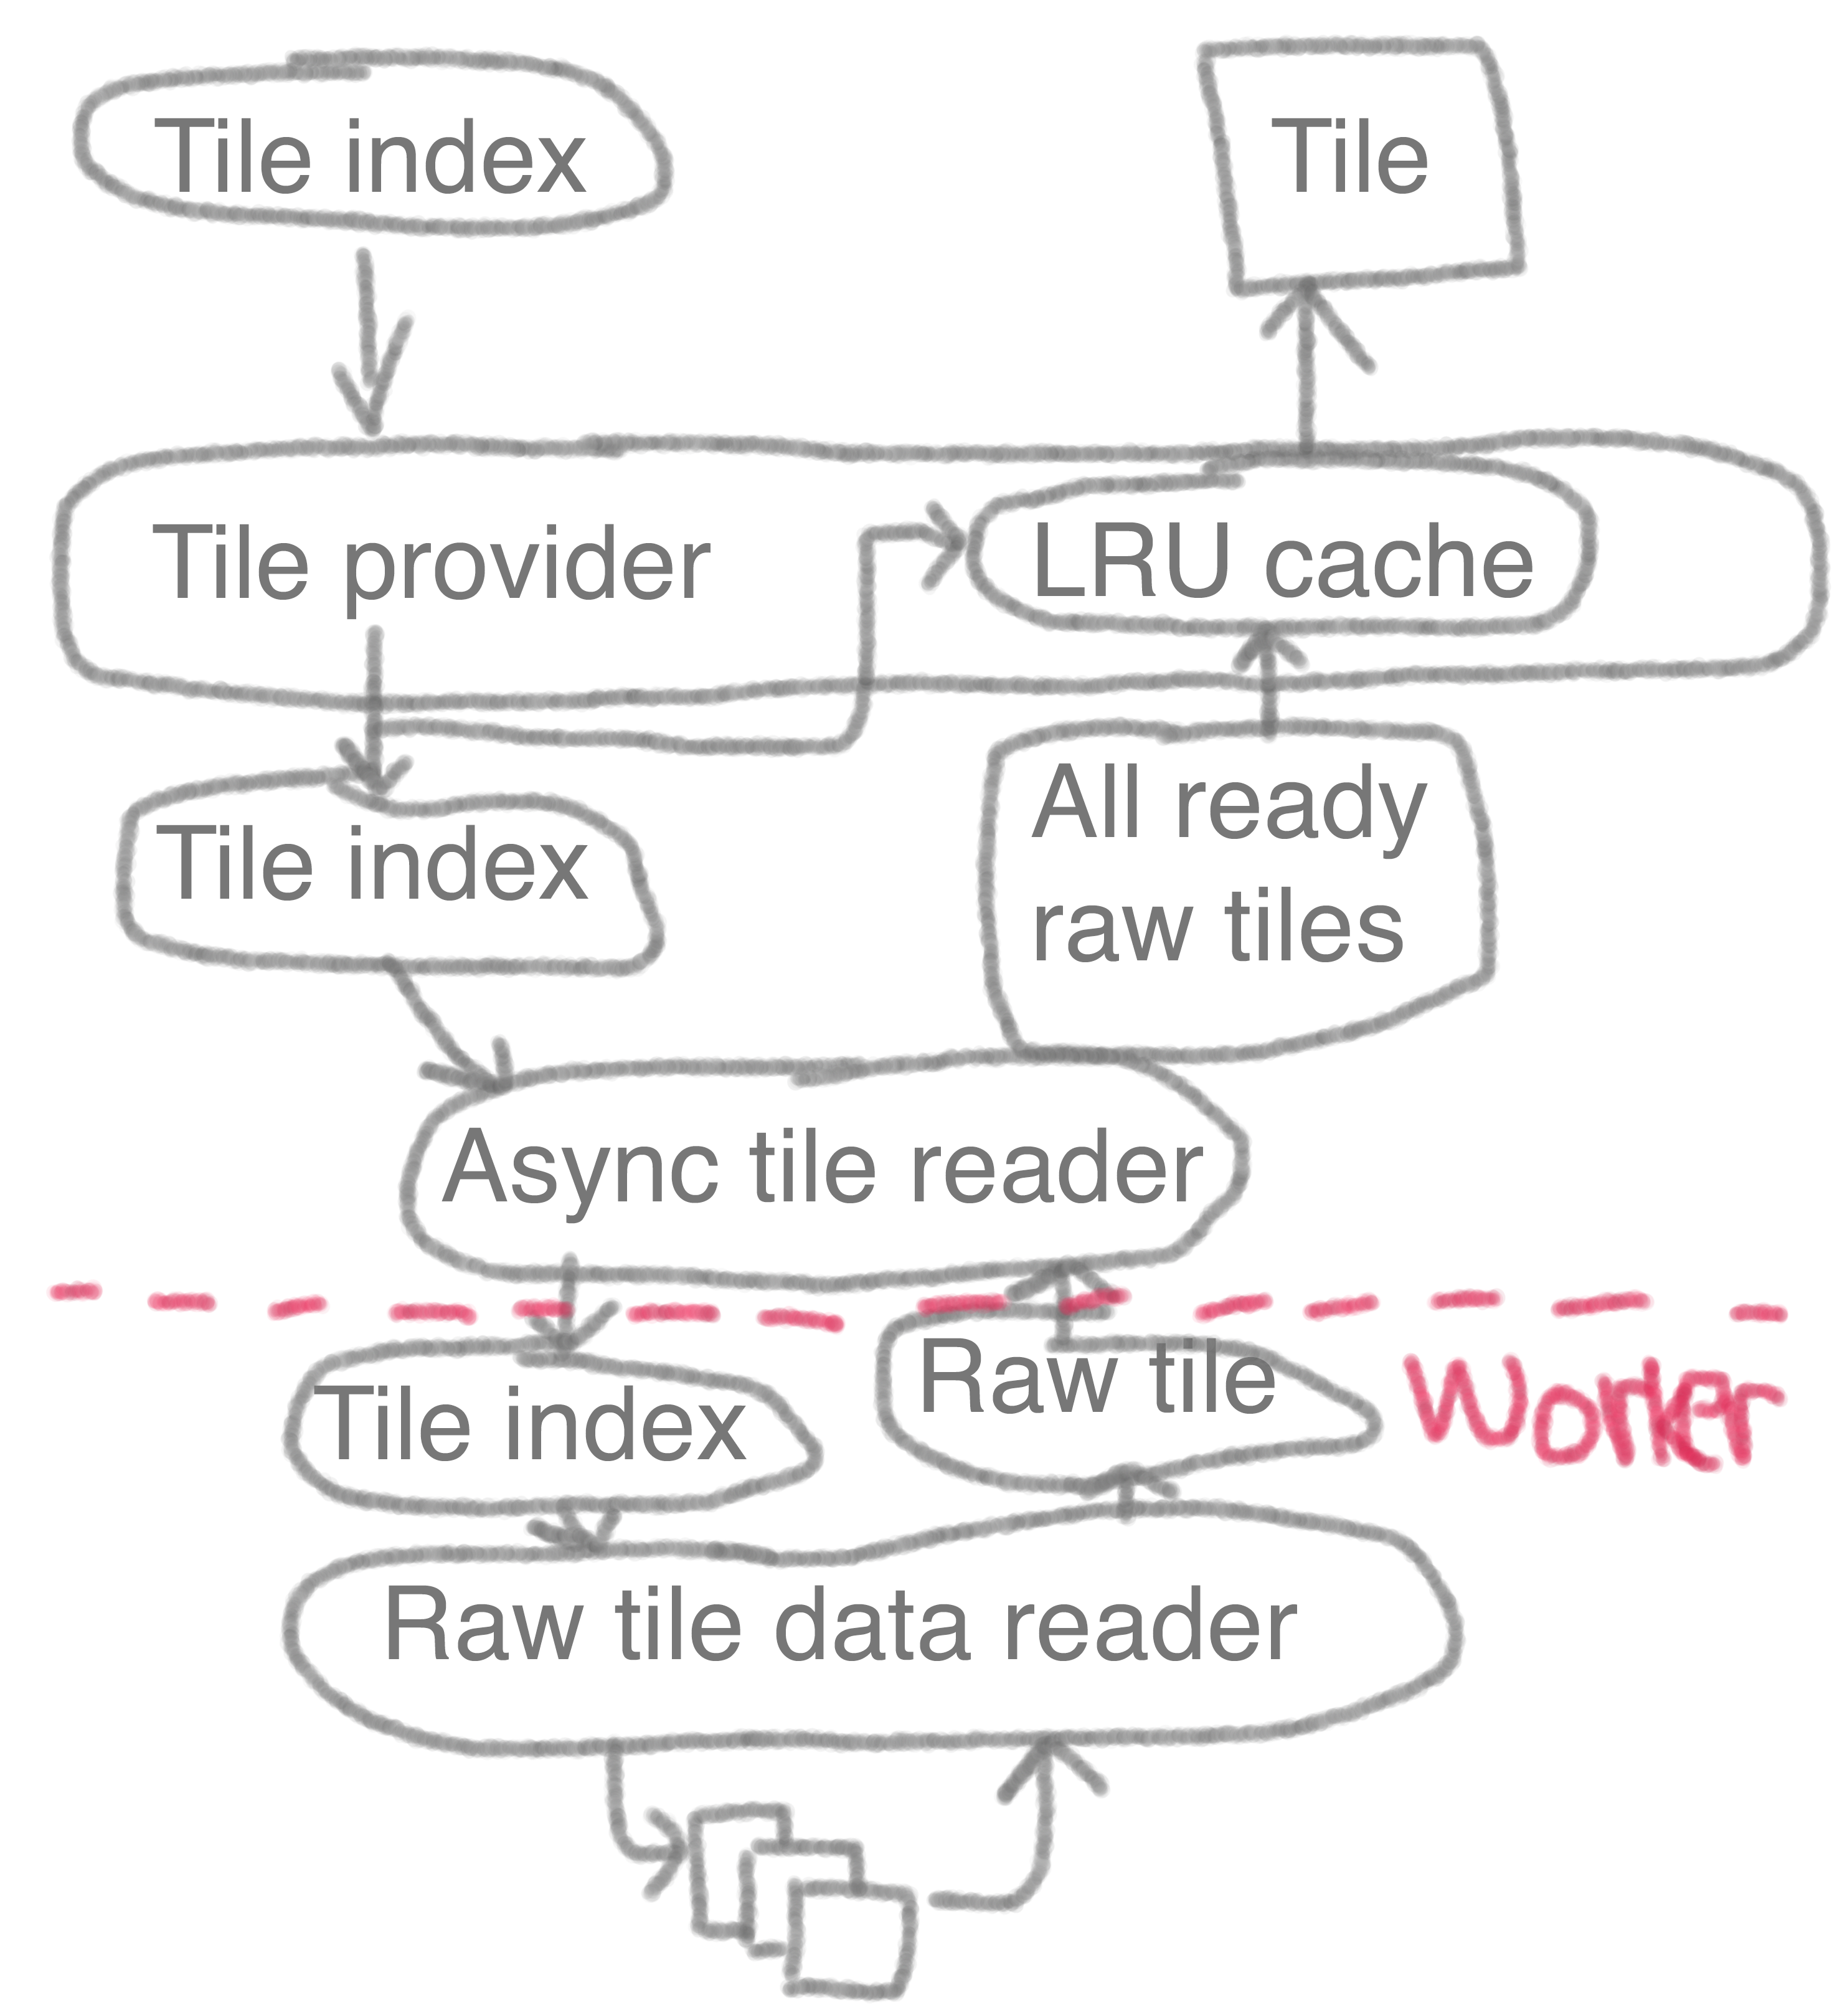
\includegraphics[width=0.5\textwidth]{figures/tile_pipeline.png}
  \caption{Tile pipeline.}
\end{figure}

\kallecomment{Figure}

\subsection{Chunk Tree}

We employ a similar chunk tree structure as described by Cozzi and Ring. (ref).
However, our version is more light weight as it does not require vertex data to be stored for every chunk node.
There are three important concepts used to update the chunk tree to achieve the highest level of detail where it is needed and avoid it where it will not make a visual difference:

\paragraph{Chunk selection} is the act of choosing whether a chunk wants to split or merge.
The evaluation is done either depending solely on the distance from the camera to the closest point on the chunk or by an approximation of the projected area of the chunk on a sphere around the camera.

\paragraph{Level limitation} is used in case a specific tile dataset does not contain any higher resolution tiles.
 To avoid unnecessary splits of chunk nodes, they should not split unless there is any higher resolution data available.

\paragraph{Chunk culling} is the act of testing every chunk if it needs to be rendered or if it is invisible.
Chunks that are behind the horizon of the globe can be culled.
So can chunks that are outside of the camera frustum.

\subsection{Chunk Rendering}

Given a valid chunk tree, each chunk needs to be rendered individually.
The downside of using a light weight chunk representation is that we are limited to the use of height mapping for vertex positioning which is done on the fly in the vertex shader.
This, however saves us from preprocessing.
This is useful since we can load height layers on demand.
We employ two different types of rendering techniques to account for both accuracy and precision.

\subsubsection{Model Space Rendering}

Using the inverse projection \kallecomment{need to define the inverse projection in overview}, vertices of a given chunk are unprojected from the georeferenced latitude-longitude projection to the model space of the globe.

This unprojection is performed in single precision on the GPU and results in the chunk being accurately mapped to the curvature of the reference ellipsoid.
 
\subsubsection{Camera Space Rendering}

The same unprojection can be performed in double precision on the CPU for the four corner points of the chunk.
These points are then transformed to camera space in double precision where they are then casted to single precision and uploaded to the GPU.
Now the rest of the vertices representing the chunk can be bilinearly interpolated for the chunk to be mapped on to the reference ellipsoid.

This method results in high precision rendering due to the origin practically being moved to the center of the camera.
The accuracy is lower however since the chunks are approximated as flat surfaces as a result of the bilinear interpolation.

\subsubsection{Combination}

To achieve both the accuracy required for the curvature and the precision required for rendering small chunks near the surface, we simply use a cutoff level where chunks below it that are big and need to be curved are rendered with the model space method and all smaller chunks which are better approximated as flat surfaces are rendered with the camera space method.

\subsubsection{Fragment Blending}

To account for versatility and seamless level switching we perform three different types of fragment blending:

\paragraph{Layer group blending} is performed so that many different layer groups can be blended together.
One important example is the use of grayscale overlays over color layers.
The grayscale overlay layer group is used to sample the underlying color (hue and saturation) and setting the lightness (value) according to the value of the grayscale overlays.

\paragraph{Layer blending} is performed so that many layers of the same layer group can be rendered together.
One example is if an overlying layer contains non unit alpha values or the ability to fade between layers using an opacity setting.

\paragraph{Level blending} is performed to achieve smooth level switching.
An interpolation parameter is calculated for each fragment depending on its distance to the camera.
This interpolation parameter is used to interpolate between the tile of the current chunk level and the corresponding tiles of the two following lower level tiles.

\subsection{Time Varying Datasets}

\subsection{Rover Locations}
\kallecomment{In case we get something to show in time}

\subsection{Atmosphere}
\kallecomment{Or not...?}

\subsection{Milti Display Systems Rendering}
\kallecomment{Clustered rendering, dome rendering, stereoscopic rendering}

\section{Conclusion} \label{sec:system}
\begin{enumerate}
  \item Blabla; introduction in reverse
  \item Future work:
  \begin{enumerate}
    \item Focus more on scientific rather than engineering goals
  \end{enumerate}
\end{enumerate}
Length: About 1 page

%% if specified like this the section will be committed in review mode
\acknowledgments{
The authors wish to thank A, B, C. This work was supported in part by
a grant from XYZ.}

%\bibliographystyle{abbrv}
\bibliographystyle{abbrv-doi}
%\bibliographystyle{abbrv-doi-narrow}
%\bibliographystyle{abbrv-doi-hyperref}
%\bibliographystyle{abbrv-doi-hyperref-narrow}

\bibliography{references}

\begin{thebibliography}{99}

\bibitem{bigdata}
\url{https://open.nasa.gov/blog/what-is-nasa-doing-with-big-data-today/}

\bibitem{mromission}
\url{http://pds-imaging.jpl.nasa.gov/portal/mro_mission.html}

\bibitem{MDIM2.1}
\url{https://astrogeology.usgs.gov/search/map/Research/ISPRS/ISPRS04_3006_B_Archinal}

\bibitem{MDIM2.1_web}
\url{https://astrogeology.usgs.gov/search/map/Mars/Viking/MDIM21/Mars_Viking_MDIM21_ClrMosaic_global_232m}

\bibitem{MOLA}
\url{https://astrogeology.usgs.gov/search/map/Mars/GlobalSurveyor/MOLA/Mars_MGS_MOLA_DEM_mosaic_global_463m}

\bibitem{HiRISE_info}
\url{https://astrogeology.usgs.gov/maps/mars-hirise-camera}

\bibitem{HiRISE_data}
\url{http://www.uahirise.org}

\end{thebibliography}

\end{document}

